\documentclass[11pt,a4paper]{book}
\usepackage[utf8]{inputenc}
\usepackage{amsmath}
\usepackage{amsfonts}
\usepackage{amssymb}
\usepackage{graphicx}
\usepackage{url}
\usepackage{lipsum}
\usepackage{marginnote}
\usepackage[disable]{todonotes}

\author{FrontEndART Szoftver Kft.}
\title{Installation Guide of the CROSSMINER Advanced Integrated Development Environments Plug-in}

\date{Version 1.15.0.rev0}

\newcommand{\todoi}[1]{\todo[inline]{#1}}

\makeatletter
\renewcommand{\maketitle}{
\vspace*{.1\textheight}
\begin{center}
	
\includegraphics[width=.6\textwidth]{pic/CROSSMINER-logo-large.png}
\end{center}
\begin{center}
	\Huge\@title
\end{center}
\vfill
\begin{center}
	\large\@author\\\@date{} $\bullet$ \today
\end{center}
}
\makeatother

\newcommand{\placeholder}[1]{$\left\langle\text{#1}\right\rangle$}

\newcommand{\SHALL}{\colorbox{red!25}{\textsc{shall}}}
\newcommand{\SHOULD}{\colorbox{orange!25}{\textsc{should}}}
\newcommand{\MAY}{\colorbox{cyan!25}{\textsc{may}}}

\newcommand{\status}[1]{\textbf{Status:} #1}
\newcommand{\todom}{\textcolor{gray}{to do}}
\newcommand{\waitingForServer}{\textcolor{red}{waiting for server side implementation}}
\newcommand{\inprogress}{\textcolor{orange}{partially done}}
\newcommand{\done}{\textcolor{green}{done}}

\newcommand{\unknown}{\colorbox{yellow}{???}}

\usepackage{ifthen}
\newboolean{showreq}
\setboolean{showreq}{false}
\newcommand{\req}[4][\todom]{
\ifthenelse{\boolean{showreq}}{
	\medskip\marginnote{
\includegraphics[width=2.75em]{pic/contract}}\noindent\textbf{\textsf{Requirement #2}} #4  \status{#1}\\\noindent\textit{#3}\bigskip\par
}{}
}

\begin{document}
	
\begin{titlepage}
	\maketitle
\end{titlepage}

\tableofcontents

\chapter{Installation guide}
Update sites are used to organize and export features so they can be installed into Eclipse applications. A feature is used to package a group of plug-ins together into a single installable and updatable unit. Features have a manifest that provides basic information about the feature and its content. content may include plug-ins, fragments and any other files that are important for the feature. A feature can also include other features. The delivery format for a feature is a JAR, but each included plug-in will be provided as a separate JAR.

\section{Create an update site with Eclipse IDE}

First of all, you need to create a feature, from our plug-in. You can create a new feature by creating a New Feature Project. After your feature project is completed, you have to add our plug-in in feature.xml Included Plug-ins tab as Figure~\ref{fig:feature} shows.

\begin{figure}[!h]
	\centering
	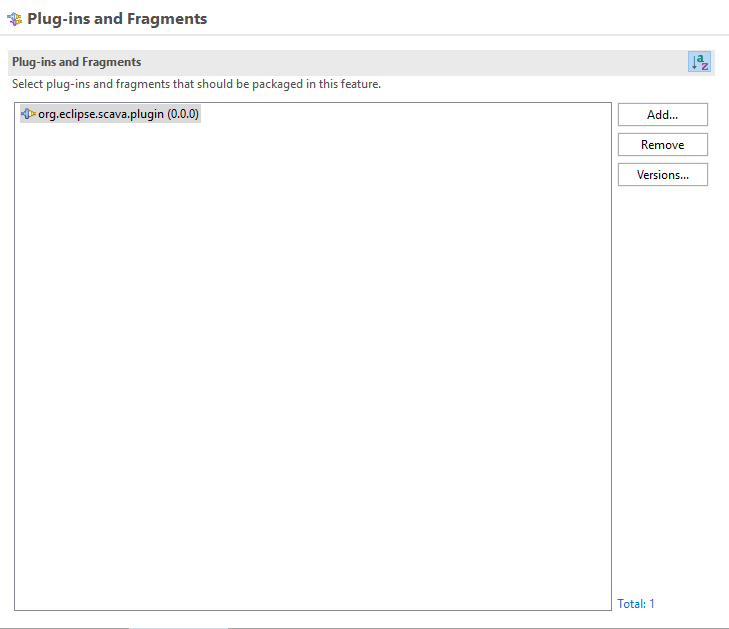
\includegraphics[width=\linewidth]{pic/feature.png}
	\caption{Included plug-ins window}
	\label{fig:feature}
\end{figure}

When your feature is ready, you have to create an update site. You can create a new update site by creating a New Update Site Project. After your update site project is completed, you have to add the feature in site.xml Site Map tab as Figure~\ref{fig:update} shows. After you added the feature to site.xml you can Build an update site.


\begin{figure}[!h]
	\centering
	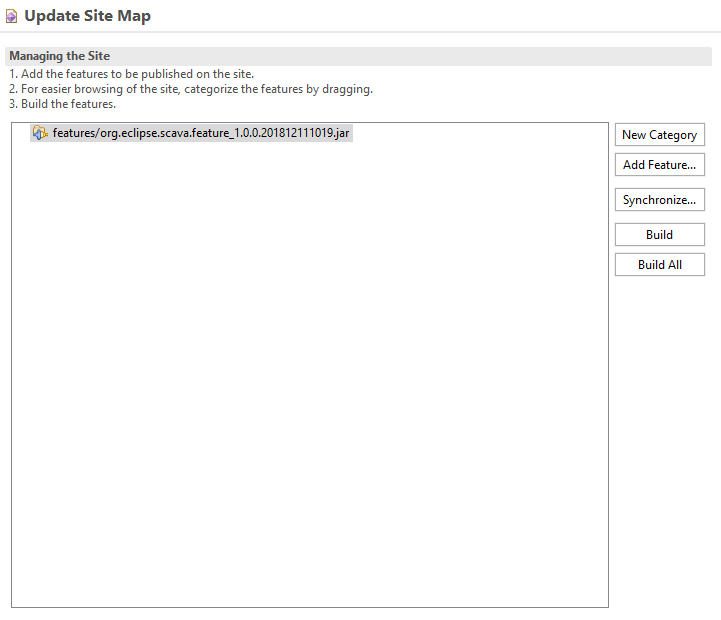
\includegraphics[width=\linewidth]{pic/update_site.png}
	\caption{Site Map window}
	\label{fig:update}
\end{figure}

\section{Install plug-in via an update site}

To install plug-in via an update site select the \textit{Install new software} under the Help menu in Eclipse. As you see on Figure~\ref{fig:install_updatesite} the following window you can choose the location of the update site. The location can be a remote or local one. After you select the update site's location it will be shown in the list. You can browse the plug-in's features and disable it if it is not necessary for you. After you are ready, click the \textit{Next} button. On the following screen you have to accept the license agreement if you want to continue the installation. The last screen you see the installation details, on this screen there is a list which contains all of the selected feature for your installation. To finish the installation process click on the \textit{Finish} button.

\begin{figure}[h]
	\centering
	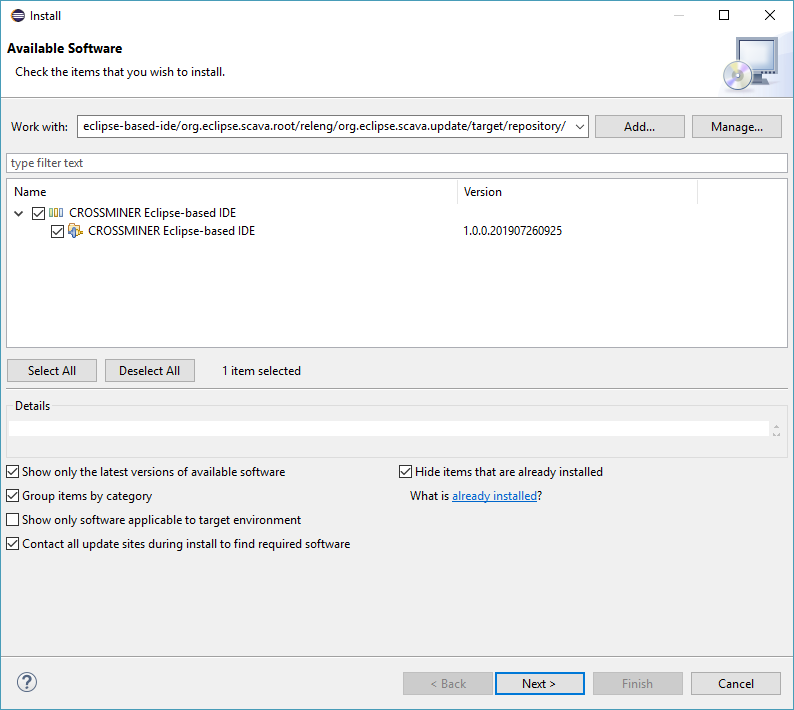
\includegraphics[width=\linewidth]{pic/updatesite.png}
	\caption{Available Software window}
	\label{fig:install_updatesite}
\end{figure}

\req[\done]{U12}{Able to obtain the API results in JSON format}{\SHALL}
\req[\done]{U13}{Able to use the API over REST}{\SHALL}
\req[\done\todo{done up to date}]{U18}{API is utilised by all UIs (dashboard, IDE plugin)}{\SHALL}

\req[\todom]{U154}{Eclipse users can invoke code recommender via an easy shortcut}{\SHALL}
\req[\todom]{U156}{Eclipse IDE proposes a dedicated view or perspective for recommendations}{\SHALL}
\req[\todom]{U158}{Eclipse IDE plugin can be installed via the Marketplace}{\SHALL}
\req[\done]{U159}{Eclipse IDE plugin can be installed via an update site}{\SHALL}

\req[\todom]{U220}{User and admin documentation is embedded into the UI}{\SHALL}
\req[\done]{U225}{Plugin supports the latest supported release of Eclipse}{\SHALL}

\req[\done\todo{up to date}]{D138}{The CROSSMINER REST API shall use UTF-8 encoding for all kind of data sent or received in text mode.}{\SHALL}


\end{document}
